\documentclass[a4paper,12pt]{article}

\usepackage[utf8]{inputenc}
\usepackage[T1]{fontenc}
\usepackage[french]{babel}
\usepackage[margin=2cm]{geometry}
\usepackage{graphicx}
\usepackage{textcomp}
\usepackage{verbatim}
\usepackage{pdfpages}
\usepackage{url}
\usepackage{hyperref}
\usepackage{tabto}
\usepackage{mathtools, bm}
\usepackage{amssymb, bm}
\usepackage{amsmath, amsfonts, amssymb}
\usepackage{float}

\hypersetup{linktoc=all}

\newcommand{\ts}{\textsuperscript}
\newcommand{\tr}{\textregistered}

\begin{document}


	%frontmatter
		\begin{titlepage}
	\begin{center}
		\vspace*{2.5cm}
		\textbf{
		\huge{
		\textsc{Rapport du projet}\\}}

		\vspace{5cm}

		\LARGE{
		\textsc{Mises en oeuvre de la méthode des éléments finis}\\[0.5\baselineskip]
		Thibault Cimic\\

		\vspace{5cm}
		\textsc{\today}\\ 

		\vspace{1cm}
		\textsc{Superviseur:\\
		X. Claeys, P. Marchand}\\

		\vspace{1cm}
		\textsc{Paris\\
		Universite Pierre et Marie Curie}\\}

		\end{center}

\end{titlepage}
		%\tableofcontents
 	  \setcounter{page}{1}
		
		
\section{Probl\`eme de Helmoltz}
\subsection{Question 1}

La première routine crée est : read(filename). Elle renvoie le tableau des noeuds et des éléments du maillage filename.\\
La deuxième routine crée est : PlotMesh(filename). Elle affiche le maillage filename comme sur la figure suivante.\\
\begin{figure}[H]
\begin{center}
        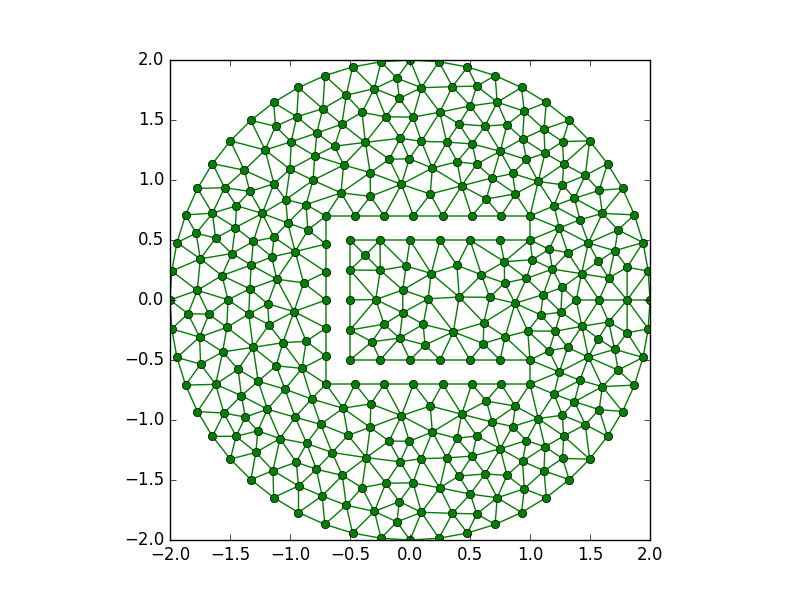
\includegraphics[scale = 0.6]{image/Maillage3/figure_1}
\end{center}
\caption{Graphique obtenu par la routine PlotMesh pour le maillage 3}
\end{figure}
L'utilisateur dipose également d'une troisième routine nommée : PlotOnMesh(f,filename, title = ""), pour son utilisation se référer au fichier README.txt.


\subsection{Question 2}

Lorsque l'on mets le problème (1) sous forme variationnelle, on trouve la forme bilinéaire symétrique suivante :
\[a:\begin{array}{ccccc}
H^{1}(\Omega)^{2} & \to & \mathbb{C}\\
(u,v) & \mapsto & \int_{\Omega}{(\nabla u \nabla v - w^{2}uv)dx}
\end{array}
\]
Cette dernière n'est alors pas nécessairement coercive. En effet, par exemple pour $w=0$ et $u \in H^{1}(\Omega)$, on a :
\[a(u,u) = ||\nabla u||^{2}_{L^{2}(\Omega)} \leq ||u||^{2}_{H^{1}(\Omega)} = ||\nabla u||^{2}_{L^{2}(\Omega)} + ||u||^{2}_{L^{2}(\Omega)}
\]
Cependant, on peut facilement trouver des conditions suffisantes pour que le problème soit coercif.
Premièrement, si $w \in i\mathbb{R}$, alors $w^{2} \in \mathbb{R}_{-}$ et on a :
\[\Re(a(u,u)) = a(u,u) \geq \min(1,-w^{2})||u||^{2}_{H^{1}(\Omega)} \]
De manière un peu plus générale, on a :
\[\Re(a(u,u)) = ||\nabla u||^{2}_{L^{2}(\Omega)} - \Re(w^{2})||u||^{2}_{L^{2}(\Omega)}
\]
Et ainsi avec l'inégalité suivante :
\[\Re(a(u,u)) \geq \min(1,- \Re(w^{2}))||u||^{2}_{H^{1}(\Omega)}
\]
On a donc que a est coercive dès que :
\[\min(1,- \Re(w^{2})) > 0 \]
\[\iff - \Re(w^{2}) > 0 \]
\[\iff \Re(w^{2}) < 0\]
\[\iff \Re(w)^{2} < \Im(w)^{2} \]
\[\iff |\Re(w)| < |\Im(w)| \]

La routine qui permet de calculer et tracer la solution du problème de Helmloltz est FiniteElementP1(filename,w,d,trace).\\


On obtient alors les tracés suivant pour $w = 5\pi$ et $d = [1,0]$ :
\begin{figure}[H]
\begin{center}
        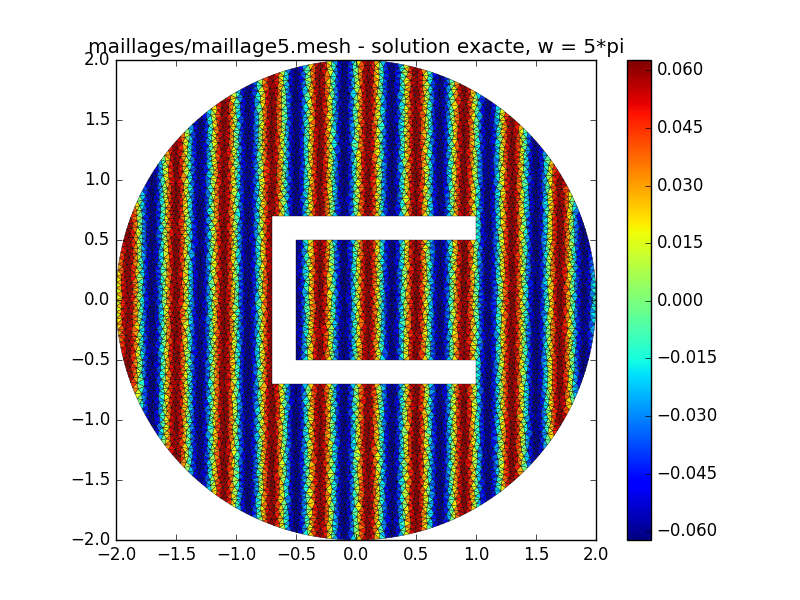
\includegraphics[scale = 0.3]{image/5Pi/figure_5}
        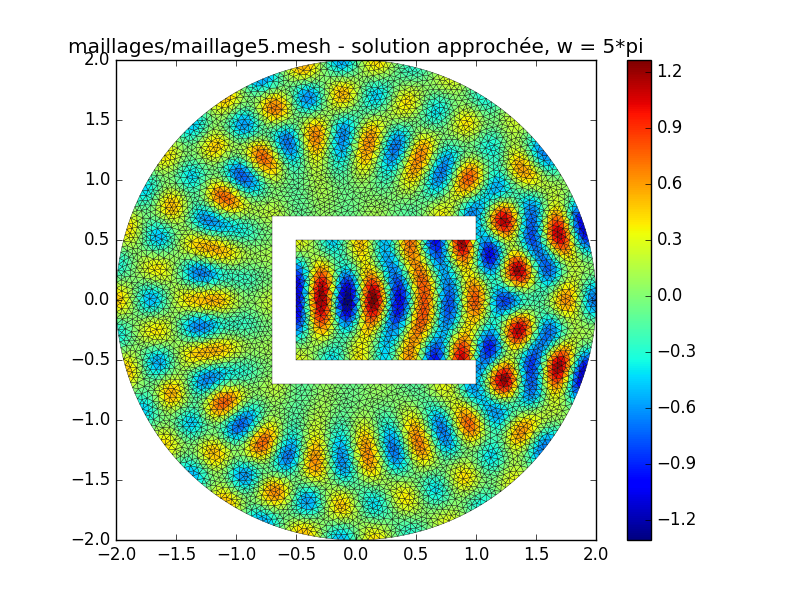
\includegraphics[scale = 0.3]{image/5Pi/figure_5-5}
        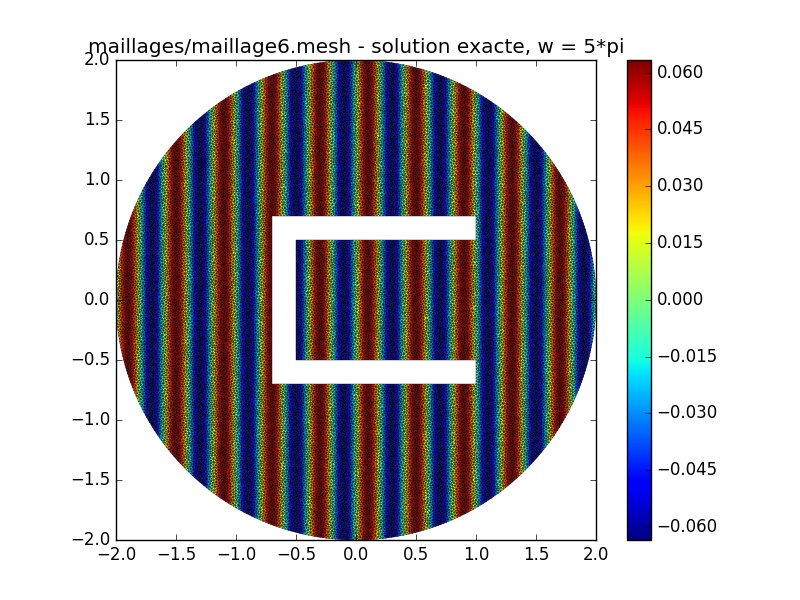
\includegraphics[scale = 0.3]{image/5Pi/figure_6}
        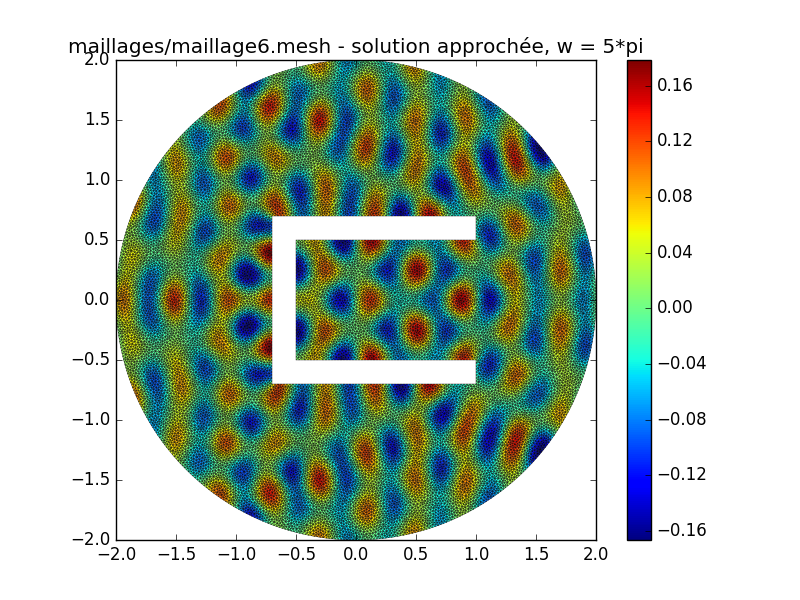
\includegraphics[scale = 0.3]{image/5Pi/figure_6-6}
        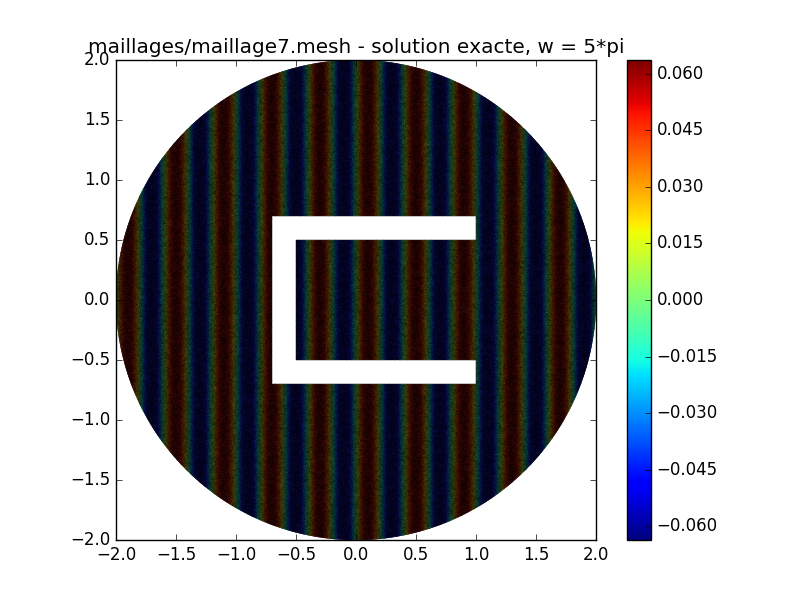
\includegraphics[scale = 0.3]{image/5Pi/figure_7}
        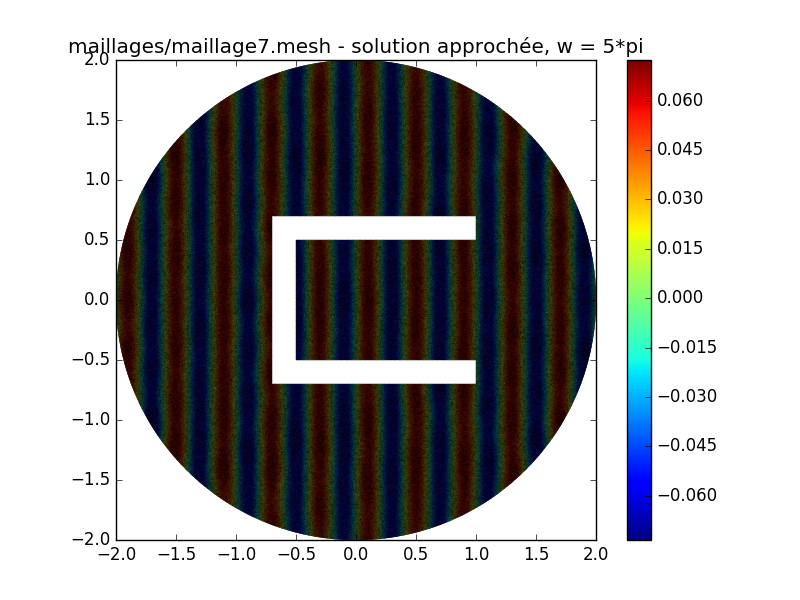
\includegraphics[scale = 0.3]{image/5Pi/figure_7-7}
\end{center}
\caption{Solution exacte et approchée pour $w = 5\pi$ pour les maillages 5 à 7}
\end{figure}

\newpage

Et voici les tracés pour $w = i$ et $d = [1,0]$ :
\begin{figure}[H]
\begin{center}
        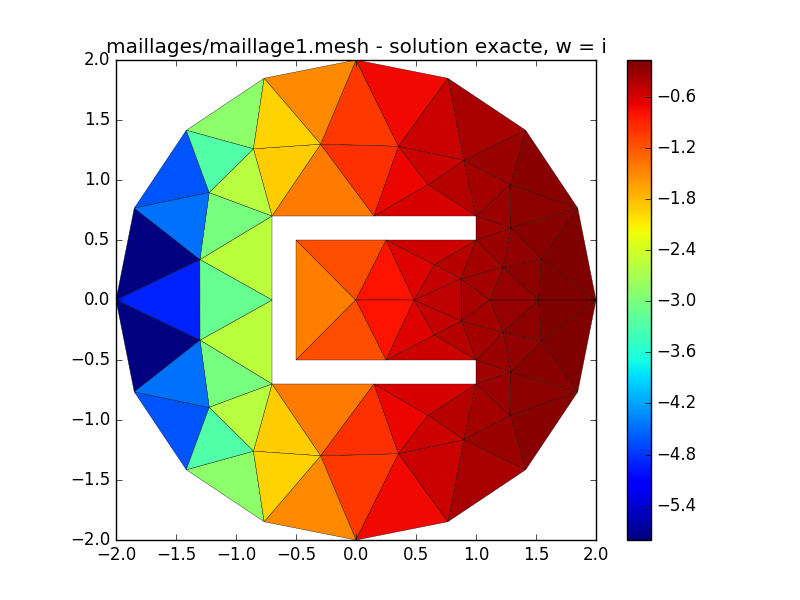
\includegraphics[scale = 0.3]{image/1j/figure_1}
        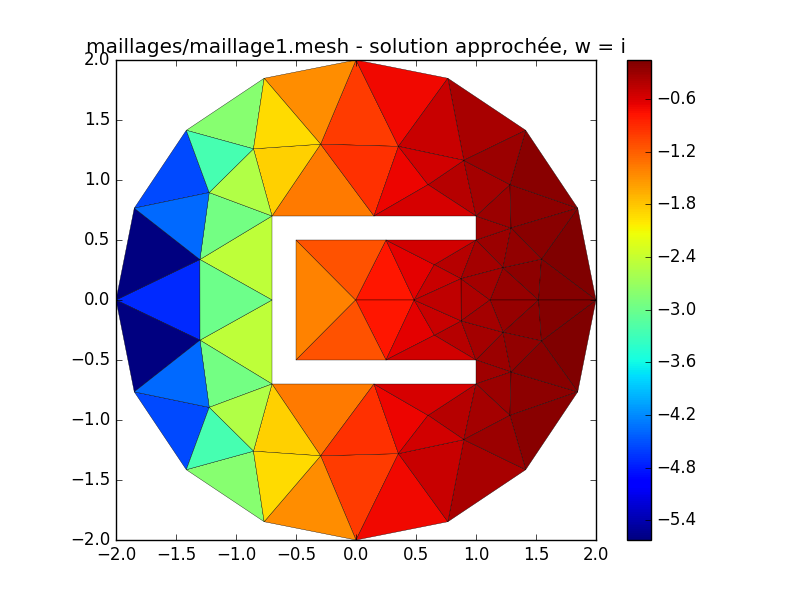
\includegraphics[scale = 0.3]{image/1j/figure_1-1}
        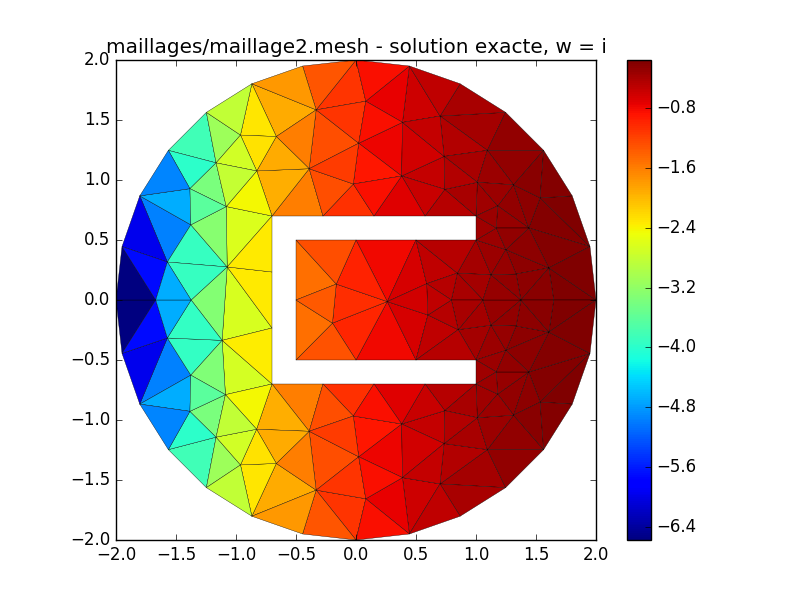
\includegraphics[scale = 0.3]{image/1j/figure_2}
        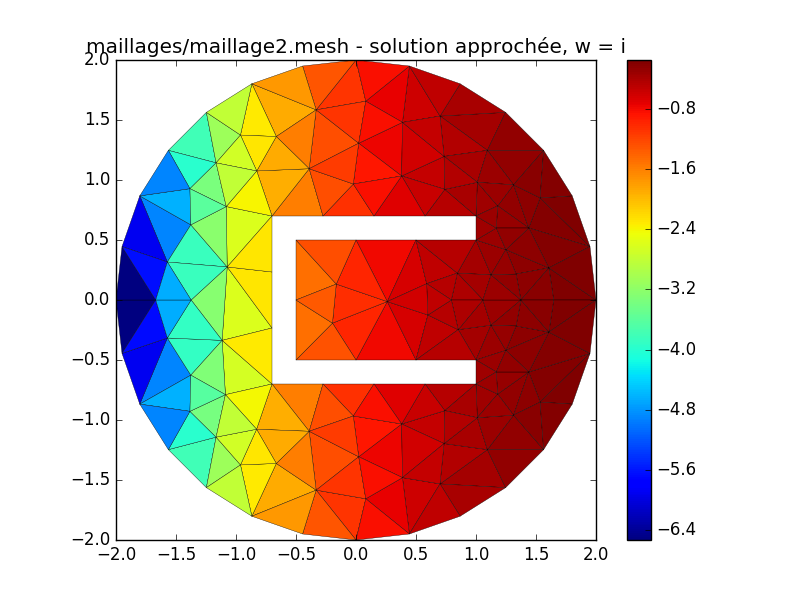
\includegraphics[scale = 0.3]{image/1j/figure_2-2}
        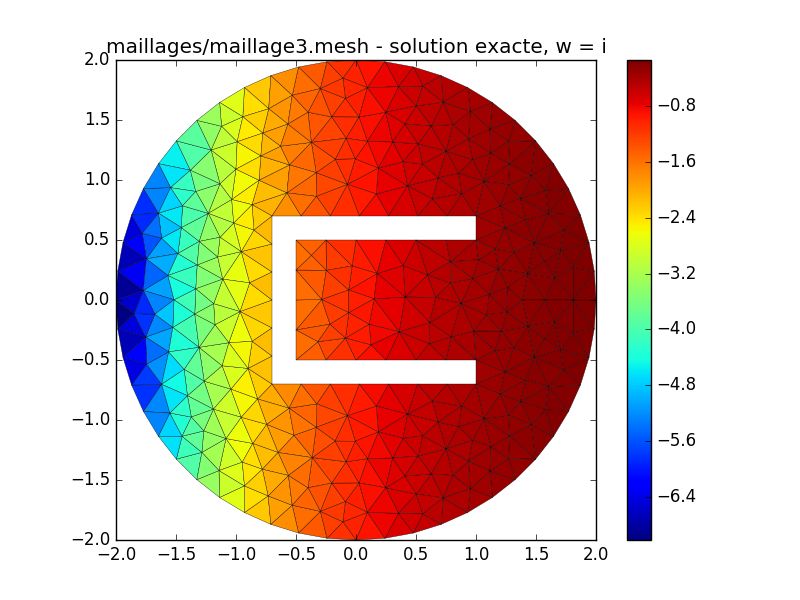
\includegraphics[scale = 0.3]{image/1j/figure_3}
        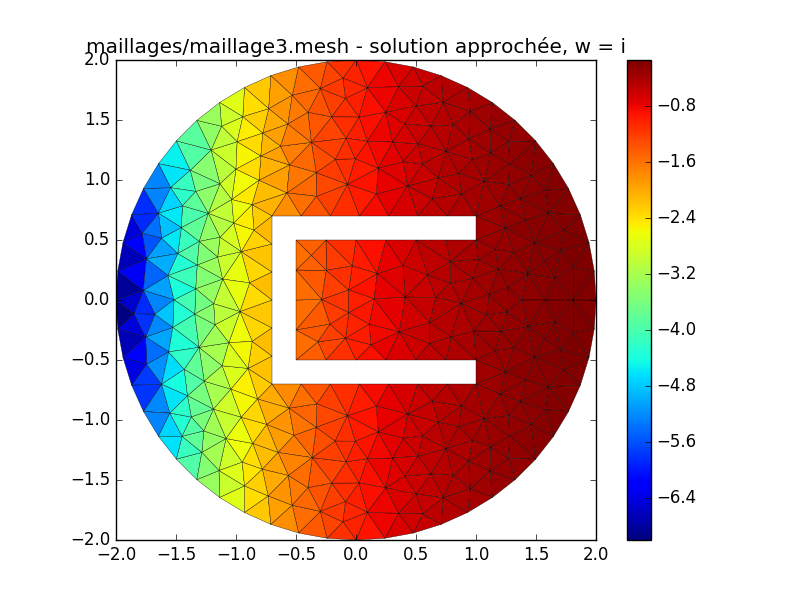
\includegraphics[scale = 0.3]{image/1j/figure_3-3}
\end{center}
\caption{Solution exacte et approchée pour $w = 5\pi$ pour les maillages 1 à 3}
\end{figure}



	
\subsection{Question 3}

Dans le cas o\`u $g(x)$ est donnée par (2), on peut chercher $u$ sous la forme :

\[u_{ref}: \begin{array}{ccccc}
\mathbb{R}^{2} & \to & \mathbb{C}\\
x & \mapsto & K\exp(iw<d,x>)
\end{array}
\]
Au quel cas en calculant le laplacien de u et en faisant le produit scalaire avec la normale extérieure unitaire on trouve que :
\[K = -\frac{i}{w}\]
et : 
\[u_{ref}: \begin{array}{ccccc}
\mathbb{R}^{2} & \to & \mathbb{C}\\
x & \mapsto & -\frac{i}{w}\exp(iw<d,x>)
\end{array}
\]

\newpage

Pour les 7 maillages donnés, le tracé de l'erreur $E(w,h)$ pour $w \in [5, 10, 20, 40, 80]$ donne :


\begin{figure}[H]
\begin{center}
        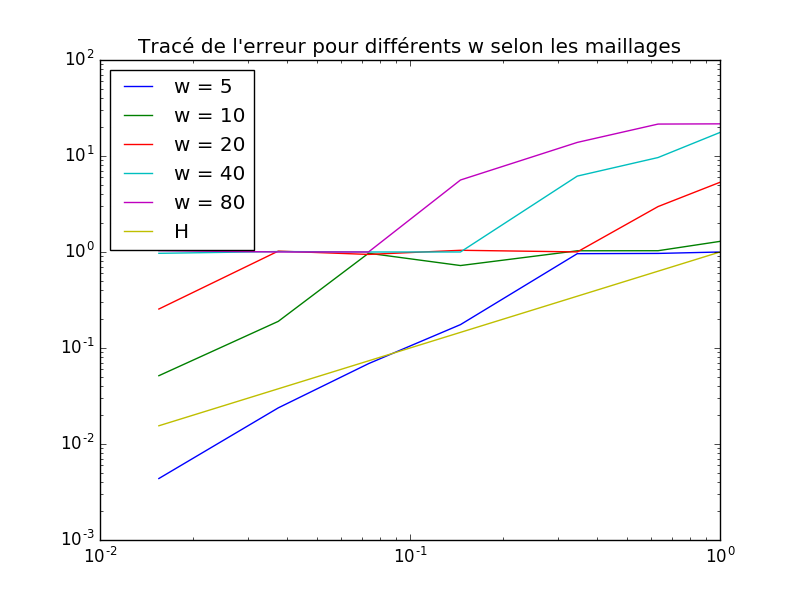
\includegraphics[scale=0.8]{image/Erreur/figure_1}
\end{center}
\caption{Tracé de l'erreur relative $E(w,h)$ pour $w \in [5, 10, 20, 40, 80]$ en échelle log-log}
\end{figure}

On voit donc que pour $w$ de plus en plus grand, l'erreur est de plus en plus importante.


\section{Ph\'enom\`ene de r\'esonnance}



\subsection{Question 4}

Pour déterminer à quelles conditions sur $\lambda \in \mathbb{C}$ existe-t-il $U \in \mathbb{R}^{N_{s}} \backslash \{0\}$ tel que :
\[
KU = \lambda MU
\]
On a les équivalences suivantes : Pour $\lambda \in \mathbb{C}$,
\begin{align*}
\exists U \in \mathbb{R}^{N_{s}} \backslash \{0\} \text{, } KU = \lambda MU & \iff \exists U \in \mathbb{R}^{N_{s}} \backslash \{0\} \text{, } \left( K-\lambda M \right) U = 0\\
& \iff  \exists U \in \mathbb{R}^{N_{s}} \backslash \{0\} \text{, } U \in \ker(K-\lambda M)\\
& \iff \ker(K-\lambda M) \ne \{0\}\\
& \iff \det(K - \lambda M) = 0
\end{align*}
Donc pour chaque $\lambda$ racine du polynôme en $X$ $det(K - X M)$, il existe $U \ne 0 \in \mathbb{R}^{N_{s}}$ solution du problème aux valeurs propres généralisées.

\newpage

Voici le tableau des 6 plus petites valeurs propres généralisées pour les 7 maillages donnés.

\begin{table}[htbp]
\centering
\caption{Tableaux des valeurs propres pour les maillages 1 à 7}
\begin{tabular}{|l|l|l|l|l|l|l|}
\hline
 & \multicolumn{1}{r|}{1} & \multicolumn{1}{r|}{2} & \multicolumn{1}{r|}{3} & \multicolumn{1}{r|}{4} & \multicolumn{1}{r|}{5} & \multicolumn{1}{r|}{6} \\ \hline
Maillage 1 & -0.0 & 0.376 & 0.52 & 1.174 & 2.236 & 2.267 \\ \hline
Maillage 2 & -0.0 & 0.361 & 0.489 & 1.108 & 2.098 & 2.179 \\ \hline
Maillage 3 & 0.0 & 0.355 & 0.476 & 1.078 & 2.034 & 2.135 \\ \hline
Maillage 4 & -0.0 & 0.347 & 0.465 & 1.052 & 2.005 & 2.114 \\ \hline
Maillage 5 & 0.0 & 0.344 & 0.462 & 1.046 & 1.997 & 2.109 \\ \hline
Maillage 6 & 0.0 & 0.344 & 0.461 & 1.043 & 1.995 & 2.108 \\ \hline
Maillage 7 & 0.0 & 0.343 & 0.46 & 1.042 & 2.107 & 1.994 \\ \hline
\end{tabular}
\label{}
\end{table}

\subsection{Question 5}

Pour le 5 ième maillage donné, lorsque l'on détermine les 6 plus petites racines de ce polynôme, on obtient les solutions $U$ suivantes :

\begin{figure}[H]
\begin{center}
        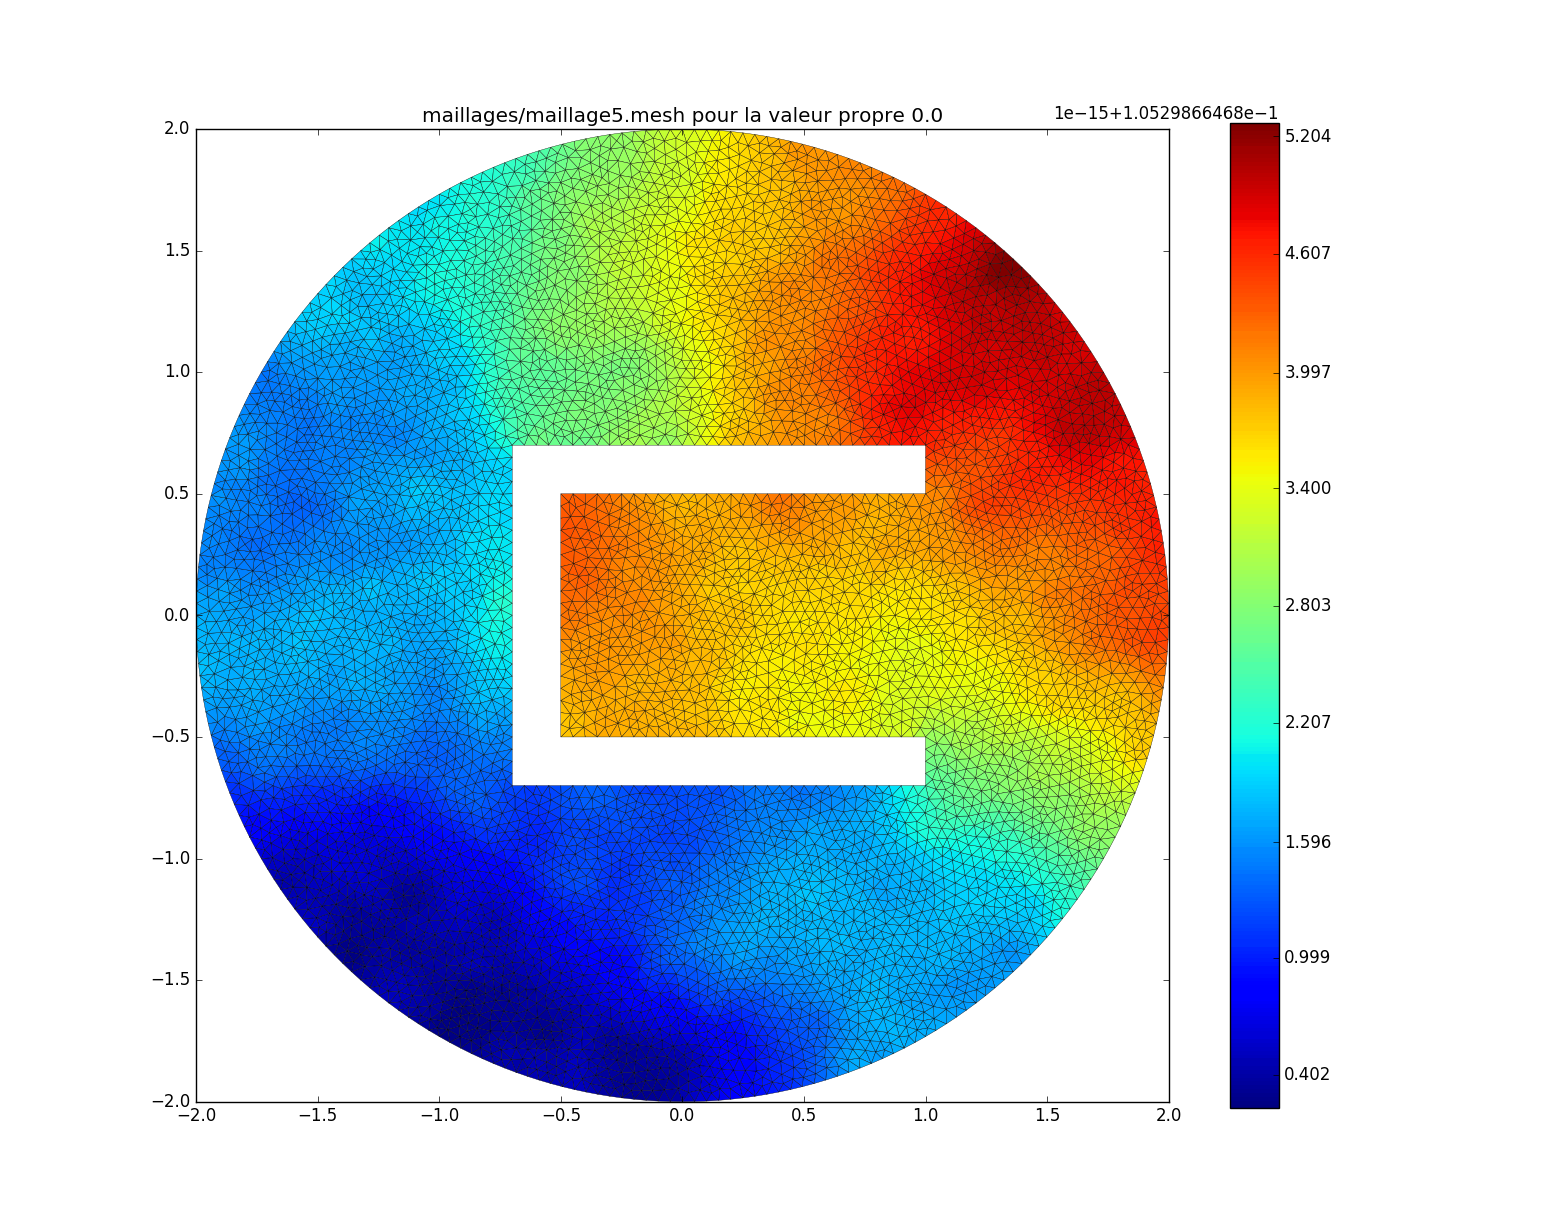
\includegraphics[scale = 0.15]{image/II/trace_1}
        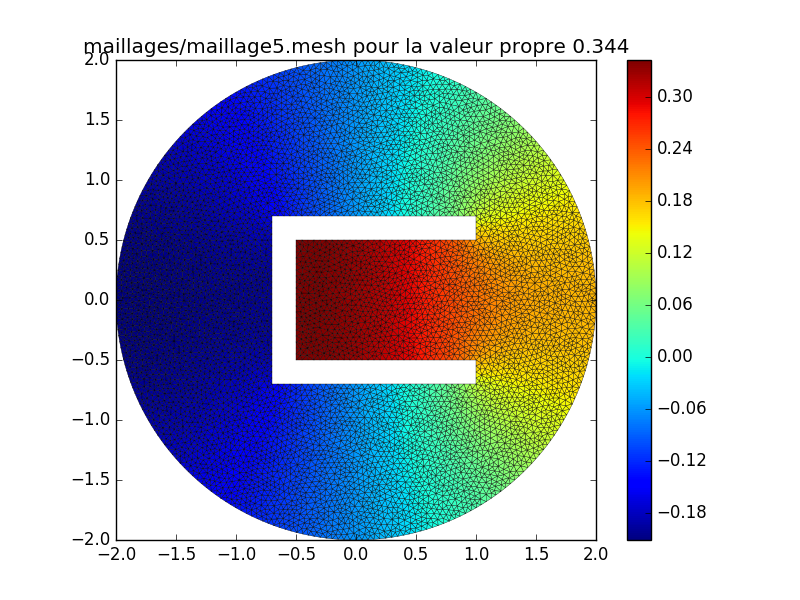
\includegraphics[scale = 0.3]{image/II/trace_2}
        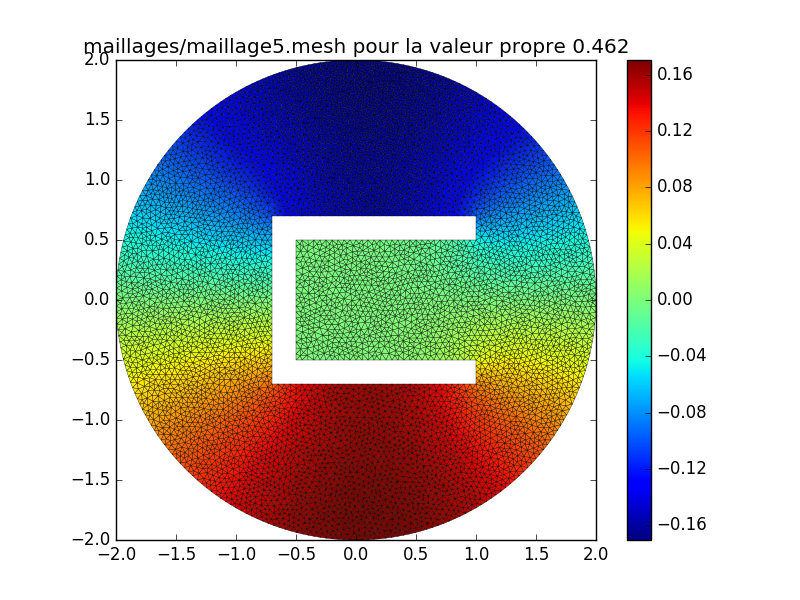
\includegraphics[scale = 0.3]{image/II/trace_3}
        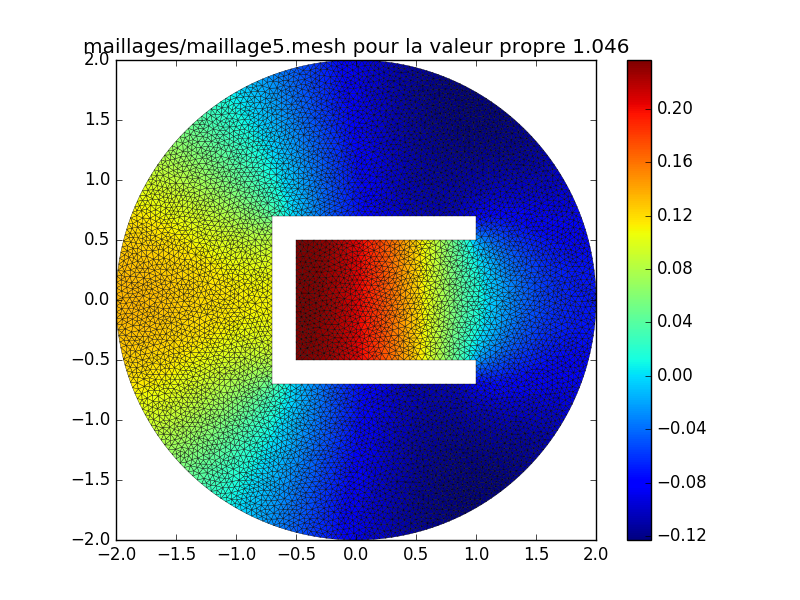
\includegraphics[scale = 0.3]{image/II/trace_4}
        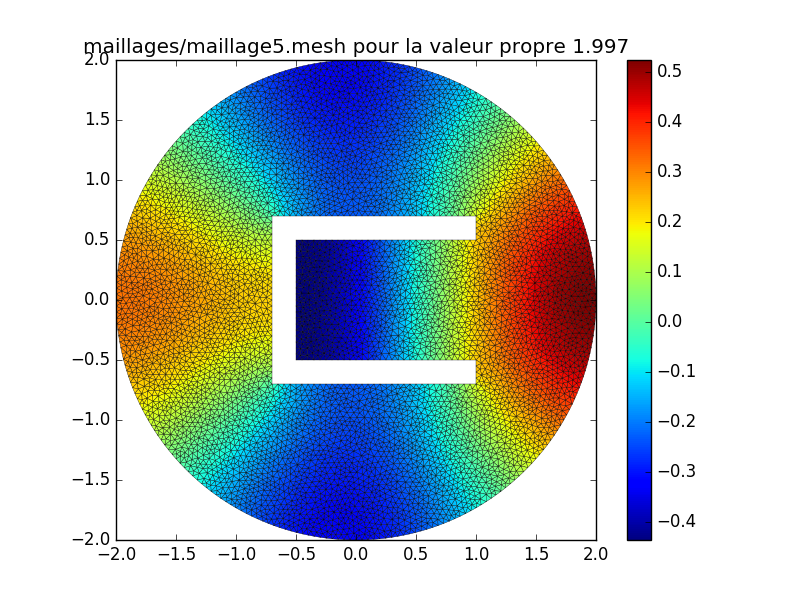
\includegraphics[scale = 0.3]{image/II/trace_5}
        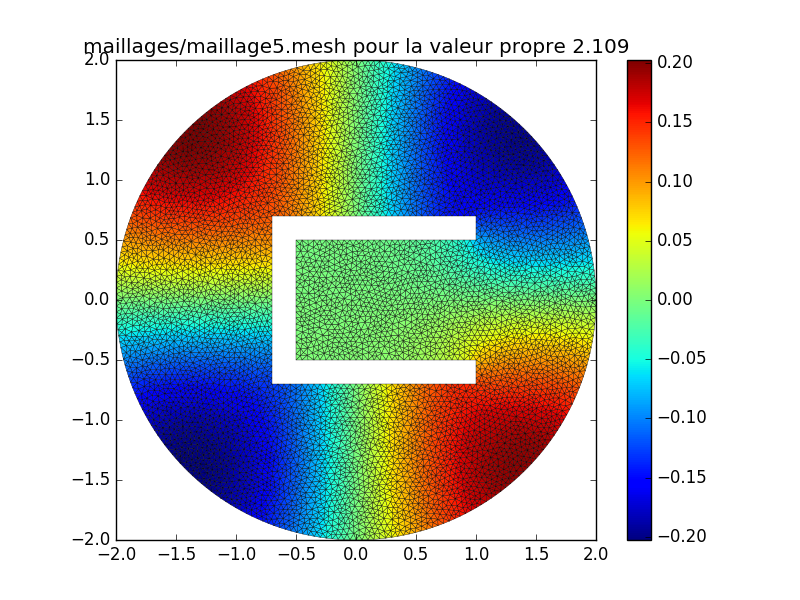
\includegraphics[scale = 0.3]{image/II/trace_6}
\end{center}
\caption{Solution approchée pour les 6 plus petites valeurs propres du maillages 5}
\end{figure}

\end{document}

